\documentclass{article}
\usepackage[utf8]{inputenc}
\usepackage{graphicx}
\usepackage{float}
\usepackage{hyperref}
\usepackage{titling}

\usepackage[scale=0.8, bmargin=2cm, tmargin=2cm, lmargin=3cm, rmargin=3cm]{geometry}

\begin{document}

\title{\textbf{Rapport projet TSMA \\
Classification Audio}}
\author{Guillaume Almyre, Pierre Célor et Antoine Pirrone}



\date{\today}
\pretitle{%
  \begin{center}
  \LARGE
  
\includegraphics[scale=0.3]{assets/ub_logo.jpg}\\[\bigskipamount]
  \vspace{3cm}
}
\posttitle{\end{center}}
\maketitle

\newpage

\section*{Introduction}

Le but de ce projet était d'implémenter un classifieur de musique en utilisant une bibliothèque de machine learning/deep learning de notre choix. Nous avons choisi d'explorer la piste des Réseaux de Neurones, et la bibliothèque que nous avons choisi d'utiliser est \textbf{TensorFlow} en Python, couplée à la bibliothèque \textbf{Librosa} pour l'extraction des features audio.\\

Notre projet s'organise de la façon suivante :

\begin{itemize}
  
\item \textbf{extract.py} : extrait les features (cf partie Choix Techniques) et les sauvegarde. L'extraction de features est très longue (quelques heures pour tout extraire de la base de morceaux de musique fournie), donc nous ne voulions pas le refaire à chaque entrainement.
  
\item \textbf{train.py} : génère le réseau de neurones avec tensorflow et l'entraine. Ce programme prend directement en entrée les fichiers de features extraits par \textbf{extract.py}

\item \textbf{sample.py} : programme pour échantillonner un modèle entrainé, évalue la classe d'un ou plusieurs fichier audio passé en paramètres (sauvegarde au passage les features extraites, pour gagner du temps plus tard)

\item \textbf{sampleFromFeatures.py} : même chose que \textbf{sample.py} mais à partir de fichiers de features précedemment sauvegardées

\item \textbf{reformat.sh} : petit script pour formater la sortie de \textbf{sampleFromFeatures.py} dans le bon format pour le challenge kaggle
  
\end{itemize}

\section*{Choix des descripteurs}

Dans \textbf{extract.py}, on extrait les features (descripteurs) suivantes par morceau grâce à \textbf{Librosa}:

\begin{itemize}

  \item \textbf{mfcc} : Mel-frequency cepstral coefficients 
  \item \textbf{chroma\_stft} : "Chromagramme" de la  Short Term Fourier Transform
  \item \textbf{melspectrogram} : Spectrogramme sur une échelle de Mel
  \item \textbf{spectral\_contrast} : contraste spectral (spectral contrast)
  \item \textbf{tonnez} : centroïde tonal (tonal centroid)
    
\end{itemize}

%% Décrire les features

\section*{Description du modèle}

Nous avons implémenté un simple réseau de neurones entièrement connecté avec deux couches cachées de 200 et 300 neurones. Le réseau prends en entrée un vecteur contenant toutes les features du morceau (on extrait le même nombre de features pour chaque morceau), et sort une probabilité d'appartenance à chaque classe dans la couche de sortie (8 neurones).\\

Lors de nos expérimentations et recherches, nous avons trouvé qu'il était très important de standardiser (normaliser) les features pour rendre le processus d'apprentissage plus efficace, car les valeurs des features peuvent beaucoup varier entre elles, et nous ne voulons pas qu'une feature prenne le dessus sur toutes les autres. Un autre argument pour cette normalisation est que la descente de gradient (que nous utilisons pour l'entrainement du réseau) converge beaucoup plus rapidement avec des dimensions normalisées \cite{DBLP:journals/corr/IoffeS15}. Nous utilisons donc \textit{StandardScaler()} de la bibliothèque \textbf{sklearn} sur nos vecteurs de features. Grâce à cette étape de standardisation, nous avons gagné en rapidité et en qualité de convergence.

%% Parler de batch size (pourquoi batchs etc)

Un autre paramètre sur lequel nous avons pu jouer est le "learning rate" (rythme d'apprentissage), qui correspond à la taille des pas de l'algorithme de descente de gradient. Ce paramètre est important car il affecte la qualité de la convergence, avec un learning rate trop grand, on risque de se retrouver dans un minimum local éloigné du minimum local, alors qu'avec un learning rate plus petit, on effectue des plus petits pas, donc on calcule une meilleure approximation du gradient, donc une meilleure convergence vers le minimum global, au prix d'un temps d'exécution plus long.

%% taille du réseau (trop grand, pas de généralisation, trop petit pas assez de mémoire ...)
%% Initialisation des poids -> normal vs xavier

%% cross validation

%% parler du matériel sur lequel a été fait l'entrainement

\section*{Résultats}


\begin{figure}[h]
  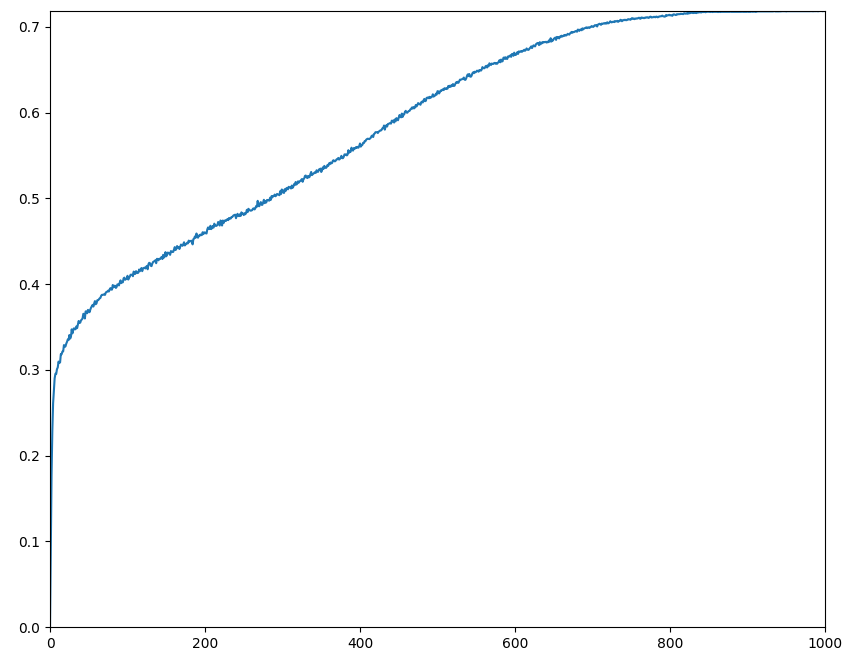
\includegraphics[scale=0.264]{assets/acc}
  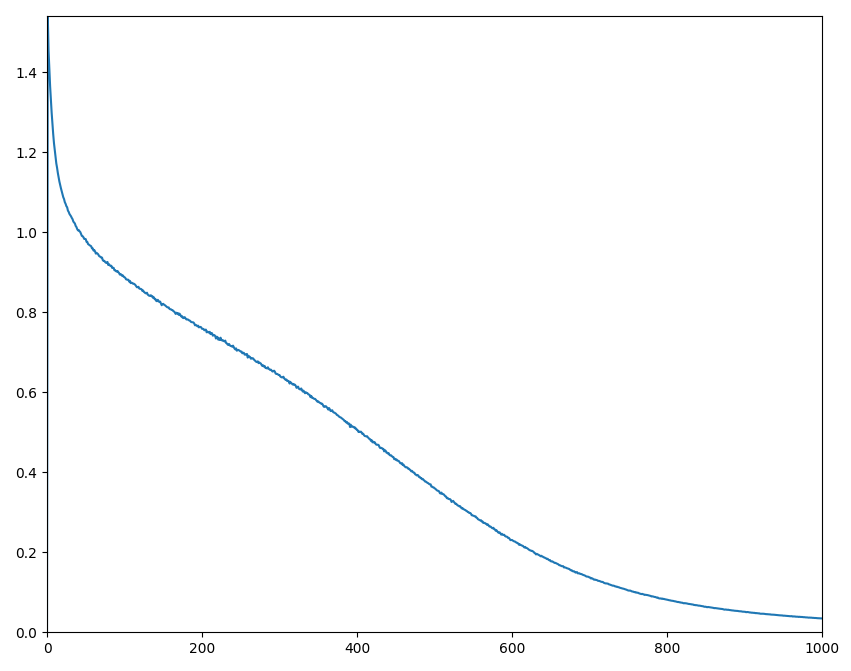
\includegraphics[scale=0.265]{assets/loss}
  
  \caption{À gauche, la précision (accuracy) du modèle pendant l'entrainement. À droite, son erreur (cost)}
  \label{acc_los}
\end{figure}

\section*{Améliorations possibles}

%% CNN ?
%% 

\section*{Conclusion}

\bibliographystyle{unsrt}
\bibliography{refs}

\end{document}
